% tcm-no-ua.tex

\documentclass{standalone}
\usepackage{tikz}

\usetikzlibrary{shapes, positioning, arrows.meta, decorations.pathmorphing}

\begin{document}
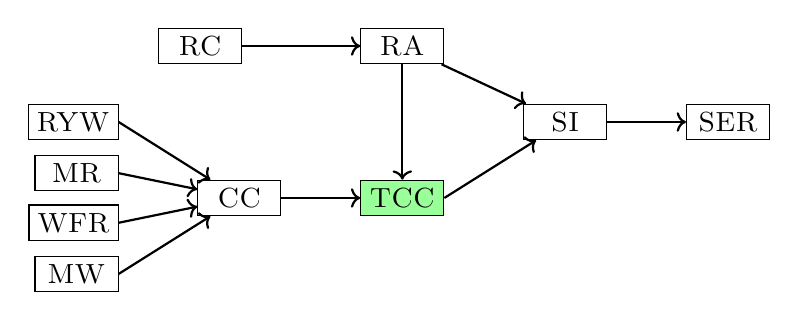
\begin{tikzpicture}[
	tcm/.style = {draw, rectangle,
	  inner sep = 3pt,
    minimum width = 30pt
    },
	]
  \node[tcm] (si) {\textsc{SI}};
  \node[tcm, right = 1.00cm of si] (ser) {\textsc{SER}};

  \node[tcm, above left = 0.50cm and 1.00cm of si] (ra) {\textsc{RA}};
  \node[tcm, fill = green!40, below left = 0.50cm and 1.00cm of si] (tcc) {\textsc{TCC}};

  % \node[tcm, left = 1.00cm of ua] (ra) {\textsc{RA}};
  \node[tcm, left = 1.00cm of tcc] (cc) {\textsc{CC}};

  \node[tcm, left = 1.50cm of ra] (rc) {\textsc{RC}};

  \node[tcm, above left = 0.50cm and 1.00cm of cc] (ryw) {\textsc{RYW}};
  \node[tcm, above left = -0.15cm and 1.00cm of cc] (mr) {\textsc{MR}};
  \node[tcm, below left = -0.15cm and 1.00cm of cc] (wfr) {\textsc{WFR}};
  \node[tcm, below left = 0.50cm and 1.00cm of cc] (mw) {\textsc{MW}};

  \path[->, thick]
    (rc) edge (ra)
    (ra) edge (si)
    (si) edge (ser)
    (cc) edge (tcc)
    (tcc.east) edge (si)
    (ra) edge (tcc)
    (ryw.east) edge (cc)
    (mr.east) edge (cc)
    (wfr.east) edge (cc)
    (mw.east) edge (cc);
\end{tikzpicture}
\end{document}